\documentclass[a4paper,12pt]{article} 


\usepackage[T2A]{fontenc}			
\usepackage[utf8]{inputenc}			
\usepackage[english,russian]{babel}	

\usepackage{graphicx, scalerel}    
\usepackage{wrapfig}               
\usepackage[14pt]{extsizes}        
\usepackage[warn]{mathtext}       
\usepackage{indentfirst}      
\usepackage[margin = 25mm]{geometry}
\usepackage[table,xcdraw]{xcolor} 
\usepackage{amsmath,amsfonts,amssymb,amsthm,mathtools}
\usepackage{wasysym}                
\usepackage{upgreek}                
\usepackage{caption}
\usepackage{multirow}
\captionsetup{labelsep=period}
\usepackage[font=small,labelfont=bf]{caption}
\usepackage{gensymb}
\usepackage[unicode, pdftex]{hyperref}
\usepackage{tikz}
\usetikzlibrary{positioning}
\usepackage{fancyhdr}
\pagestyle{fancy}
\setlength\fboxsep{3pt} % Отступ рамки \fbox{} от рисунка
\setlength\fboxrule{1pt} % Толщина линий рамки \fbox{}
\newcommand{\tocsection}[1]{\section*{#1} \addcontentsline{toc}{section}{#1}}
\newcommand{\tocsubsection}[1]{\subsection*{#1} \addcontentsline{toc}{subsection}{#1}}
\renewcommand{\cftsecleader}{\cftdotfill{\cftdotsep}}

\def\fillandplacepagenumber{%
	\par\pagestyle{empty}%
	\vbox to 0pt{\vss}\vfill
	\vbox to 0pt{\baselineskip0pt
		\hbox to\linewidth{\hss}%
		\baselineskip\footskip
		\hbox to\linewidth{%
			\hfil\thepage\hfil}\vss}}

\begin{document}
		\newcommand{\HRule}{\rule{\linewidth}{0.7mm}} % Defines a new command for the horizontal lines, change thickness here

\begin{center}
	\large\textbf{Московский Физико-Технический Институт}\\
	\large\textbf{(государственный университет)}
	
	\vfill
	

	
	\Large Вычислительная математика
	%----------------------------------------------------------------------------------------
	%	TITLE SECTION
	%----------------------------------------------------------------------------------------
	
	\HRule
	\\[0.4cm]
	{ \huge \bfseries Лабораторная работа №9}
	\\[0.4cm] % Title of your document
	\HRule
	\\[0.5cm]
	
	\ \\
	\textbf{\large Автор:} \\	
	\large Овсянников Михаил Б01-008\\
	\vfill
	\hspace*{-0.8 cm}
\includegraphics[width=100 pt]{./Include/frkt_logo.pdf}\\
	\large Долгопрудный, 2023
\end{center}

\thispagestyle{empty}

\newpage
\setcounter{page}{2}
\fancyfoot[c]{\thepage}
\fancyhead[L] {Лабораторная работа №9}
\fancyhead[R]{}

		\tableofcontents
		\newpage
		
		\tocsection{Цель}
		Решить краевую задачу для одномерного стационарного уравнения теплопроводности с кусочно-непрерывными коэффициентами.
			
		\tocsection{Теоретические сведения}
		\tocsubsection{Общая задача}

		Наша задача -- решить одномерное стационарное уравнение теплопроводности на отрезке $[0, 1]$:
		\begin{equation*}
			\begin{cases} 
				\frac{d}{dx}[k(x)\frac{du}{dx}] - q(x)u = -f(x), \\
				u(0) = u^0, \\
				u(1) = u^1, \\
			\end{cases} 
		\end{equation*}
		\noindent где $k(x)$, $q(x)$ и $f(x)$ -- кусочно-непрерывные коэффициенты, имеющие разрыв 1-го рода в точке $x_0$. В данной точке ставятся так называемые условия сопряжения, обеспечивающие непрерывность температуры $u$ и потока тепла $ku_x$:
		\begin{equation*}
			\begin{cases}
				u |_{x = x_0 - 0} = u |_{x = x_0 + 0}, \\
				ku_x |_{x = x_0 - 0} = ku_x |_{x = x_0 + 0}. 
			\end{cases}
		\end{equation*}
		
		
		Для решения данной задачи будем использовать метод встречных прогонок. Опишем его.
		
		
		\tocsubsection{Описание метода встречных прогонок}
		На области интегрирования введем сетку $x_l = lh$, $l = \overline{0 \div L}$, $Lh = 1$. Пусть точка разрыва расположена между узлами $l_\alpha$ и $l_\beta$. И пусть индекс $\alpha$ у чего-либо означает это <<что-то>> до точки разрыва, а $\beta$ -- после. Введем обозначения:
		\begin{itemize}
			\item $(k_\alpha)_{l \pm 1/2} = k_\alpha(x_l \pm h/2)$,
			
			\item $(k_\beta)_{l \pm 1/2} = k_\beta(x_l \pm h/2)$,
			
			\item $(q_\alpha)_l = q_\alpha(x_l)$,
			
			\item $(q_\beta)_l = q_\beta(x_l)$,
			
			\item $(f_\alpha)_l = f_\alpha(x_l)$,
			
			\item $(f_\beta)_l = f_\beta(x_l)$.
		\end{itemize}
		
		Теперь:
		\begin{equation*}
			\left(\frac{d}{dx}\left[k(x)\frac{du}{dx}\right]\right)_{x = x_l} \approx \frac{(k_\alpha)_{l+1/2}\displaystyle\frac{u_{l+1} - u_l}{h} - (k_\alpha)_{l-1/2}\displaystyle\frac{u_{l} - u_{l-1}}{h}}{h}, \;\;\; l = \overline{1 \div l_\alpha - 1}
		\end{equation*}
	
		\begin{equation*}
			\left(\frac{d}{dx}\left[k(x)\frac{du}{dx}\right]\right)_{x = x_l} \approx \frac{(k_\beta)_{l+1/2}\displaystyle\frac{u_{l+1} - u_l}{h} - (k_\beta)_{l-1/2}\displaystyle\frac{u_{l} - u_{l-1}}{h}}{h}, \;\;\; l = \overline{\l_\beta + 1 \div L - 1}
		\end{equation*}
	
		Подставим это всё дело в дифференциальное уравнение и получим систему из $L - 3$ уравнений на $L + 1$ неизвестных:
		\begin{equation*}
			\begin{cases}
				\displaystyle\frac{(k_\alpha)_{l+1/2}(u_{l+1} - u_l) - (k_\alpha)_{l-1/2}(u_{l} - u_{l-1})}{h^2} - (q_\alpha)_l u_l = -(f_\alpha)_l, \;\;\; l = \overline{1 \div l_\alpha - 1}, \\
				\displaystyle\frac{(k_\beta)_{l+1/2}(u_{l+1} - u_l) - (k_\beta)_{l-1/2}(u_{l} - u_{l-1})}{h^2} - (q_\beta)_l u_l = -(f_\beta)_l, \;\;\; l = \overline{\l_\beta + 1 \div L - 1}.
			\end{cases}
		\end{equation*}
	
		К этой системе добавим краевые условия и условия сопряжения в точке разрыва и получим систему из $L + 1$ уравнений на $L + 1$ неизвестных.
		
		Для упрощения записи введем еще одну группу обозначений:
		\begin{itemize}
			\item $a_l = (k_\alpha)_{l + 1/2},$
			
			\item $b_l = -\left[(k_\alpha)_{l + 1/2} + (k_\alpha)_{l - 1/2} + (q_\alpha)_l h^2\right],$
			
			\item $c_l = (k_\alpha)_{l - 1/2}, \hspace{85mm} l = \overline{1 \div l_\alpha - 1}$
			
			\item $d_l = -(f_\alpha)_l h^2.$
		\end{itemize}
	
		\vspace{20mm}
	
		\begin{itemize}
			\item $a_l = (k_\beta)_{l + 1/2},$
			
			\item $b_l = -\left[(k_\beta)_{l + 1/2} + (k_\beta)_{l - 1/2} + (q_\beta)_l h^2\right],$
			
			\item $c_l = (k_\beta)_{l - 1/2}, \hspace{85mm} l = \overline{l_\beta + 1 \div L - 1}$
			
			\item $d_l = -(f_\beta)_l h^2.$
		\end{itemize}
		
		
		
		
		Тогда общая система уравнений выглядит очень лаконично:
		\begin{equation}
			\begin{cases}
				u_0 = u^0, \\
				a_l u_{l+1} + b_l u_l + c_l u_{l - 1} = d_l, \;\;\;\;\;\;\;\;\;\; \overline{1 \div l_\alpha - 1}, \\
				u_{l_\alpha} = u_{l_\beta}, \\
				(k_\alpha)_{l_\alpha}(u_{l_\alpha} - u_{l_\alpha - 1}) = (k_\beta)_{l_\beta}(u_{l_\beta + 1} - u_{l_\beta}), \\
				a_l u_{l+1} + b_l u_l + c_l u_{l - 1} = d_l, \;\;\;\;\;\;\;\;\;\; \overline{l_\beta + 1 \div L - 1}, \\
				u_L = u^1.
			\end{cases}
			\label{MAIN_SYS}
		\end{equation}
	
		Теперь приступаем к решению. Сначала делаем прямую прогонку. Из первого уравнения подставим $u_0$ во второе и из последнего $u_L$ в предпоследнее:
		\begin{equation*}
			\begin{cases}
				u_1 	\;\;\;\,  = \;\;\;  -\frac{a_1}{b_1} u_2 \;\;\; + \frac{d_1 - c_1 u_0}{b_1} \;\;\;\;\;\;\, = \alpha_1 u_2 + \beta_1, \\
				u_{L - 1} = -\frac{c_{L - 1}}{b_{L - 1}}u_{L - 2} + \frac{d_{L - 1} - c_{L - 1} u_L}{b_{L - 1}} = \alpha_{L - 1} u_{L - 2} + \beta_{L - 1}
			\end{cases}
		\end{equation*}
		
		По индукции доказываем, что подсистемы самой системы \eqref{MAIN_SYS} сводятся к системам с двухдиагональной матрицей. Уравнения выглядят так:
		\begin{equation}
			\begin{cases}
				u_{l - 1} = \alpha_{l - 1} u_l + \beta_{l - 1}, \;\;\; l = \overline{1 \div l_\alpha - 1} \\
				u_{l + 1} = \alpha_{l + 1} u_l + \beta_{l + 1}, \;\;\; l = \overline{L - 1 \div l_\beta + 1}
			\end{cases}
			\label{BACKWARD}
		\end{equation}
		
		Прогоночные коэффициенты определяются следующим образом:
		\begin{itemize}
			\item $\alpha_l = -\displaystyle\frac{a_l}{b_l + c_l \alpha_{l-1}},$
			
			\item $\beta_l  =  \displaystyle\frac{d_l - c_l \beta_{l-1}}{b_l + c_l \alpha_{l - 1}}, \;\;\;\;\;\;\;\; l = \overline{2 \div l_\alpha - 1}$
		\end{itemize}
		
		\vspace{20mm}
		
		\begin{itemize}
			\item $\alpha_l = -\displaystyle\frac{c_l}{b_l + a_l \alpha_{l+1}},$
			
			\item $\beta_l  =  \displaystyle\frac{d_l - a_l \beta_{l+1}}{b_l + a_l \alpha_{l + 1}}, \;\;\;\;\;\;\;\; l = \overline{L - 2 \div l_\beta + 1}$
		\end{itemize}		
		
		
		\newpage
		Теперь разберемся с $l_{\alpha} - 1$, $l_\alpha$, $l_\beta$ и $l_{\beta} + 1$ уравнениями системы.
		\begin{equation*}
			\begin{cases}
				u_{l_\alpha - 1} = \alpha_{l_\alpha - 1} u_{l_\alpha} + \beta_{l_\alpha - 1}, \\
				u_{l_\alpha} = u_{l_\beta}, \\
				(k_\alpha)_{l_\alpha}(u_{l_\alpha} - u_{l_\alpha - 1}) = (k_\beta)_{l_\beta}(u_{l_\beta + 1} - u_{l_\beta}), \\
				u_{l_\beta  + 1} = \alpha_{l_\beta  + 1} u_{l_\beta}  + \beta_{l_\beta  + 1}.
			\end{cases}
		\end{equation*}
		
		По сути, последнее -- система из 4-х уравнений на 4 неизвестные. Решаем ее и получаем следующее:
		\begin{equation*}
			\begin{cases}
				u_{l_\alpha} = u_{l_\beta} = \displaystyle\frac{(k_\alpha)_{l_\alpha}\beta_{l_\alpha - 1} + (k_\beta)_{l_\beta}\beta_{l_\beta + 1}}{(k_\alpha)_{l_\alpha}(1 - \alpha_{l_\alpha - 1}) + (k_\beta)_{l_\beta} (1 - \alpha_{l_\beta + 1})}, \\
				
				u_{l_\alpha - 1} = \alpha_{l_\alpha - 1} u_{l_\alpha} + \beta_{l_\alpha - 1}, \\
				u_{l_\beta + 1} = \alpha_{l_\beta + 1} u_{l_\beta} + \beta_{l_\beta + 1}.
			\end{cases}
		\end{equation*}
		
		Этим заканчивается прямая прогонка. По уравнениям \eqref{BACKWARD} производим обратную прогонку, и таким образом решаем поставленную задачу.
		
		Всё это выглядит очень перегружено и может быть сразу непонятно, но в коде это выглядит более менее понятно.
		
		
		
		
		
		\newpage
		\tocsection{Непосредственно задача}
		\tocsubsection{Постановка задачи}
		В качестве краевой задачи был выбран номер \textbf{Вариант 3 №16} лабораторной работы №4 книги В.В.Демченко <<Вычислительный практикум по прикладной математики>>:
		\begin{equation*}
			\frac{d}{dx}\left[k(x)\frac{du}{dx}\right] - q(x)u = -f(x),
		\end{equation*}
		\noindent где:
		\begin{itemize}
			\item $u(0) = 2; \;\;\; u(1) = 1$
			
			\item $x_0 = 1/\sqrt{3}$ 
		\end{itemize}
	
		\begin{equation*}
			\begin{cases}
				k(x) = e^{-x}, \\
				q(x) = x^3, \;\;\;\;\;\;\;\;\;\; x < x_0 \\
				f(x) = x^2 - 1,
			\end{cases}
		\end{equation*}
		
		
		\begin{equation*}
			\begin{cases}
				k(x) = e^{-x}, \\
				q(x) = x, \;\;\;\;\;\;\;\;\;\; x > x_0 \\
				f(x) = 1,
			\end{cases}
		\end{equation*}
		
		
		Что-то придумывать не будем и просто реализуем всё это в программном виде.
		
		
		\newpage
		\tocsubsection{Результаты}		
		
		Само решение выглядит довольно гладким, и кажется, что условия сопряжения на разрыве соблюдены.
		\begin{figure}[h!]
			\centering
			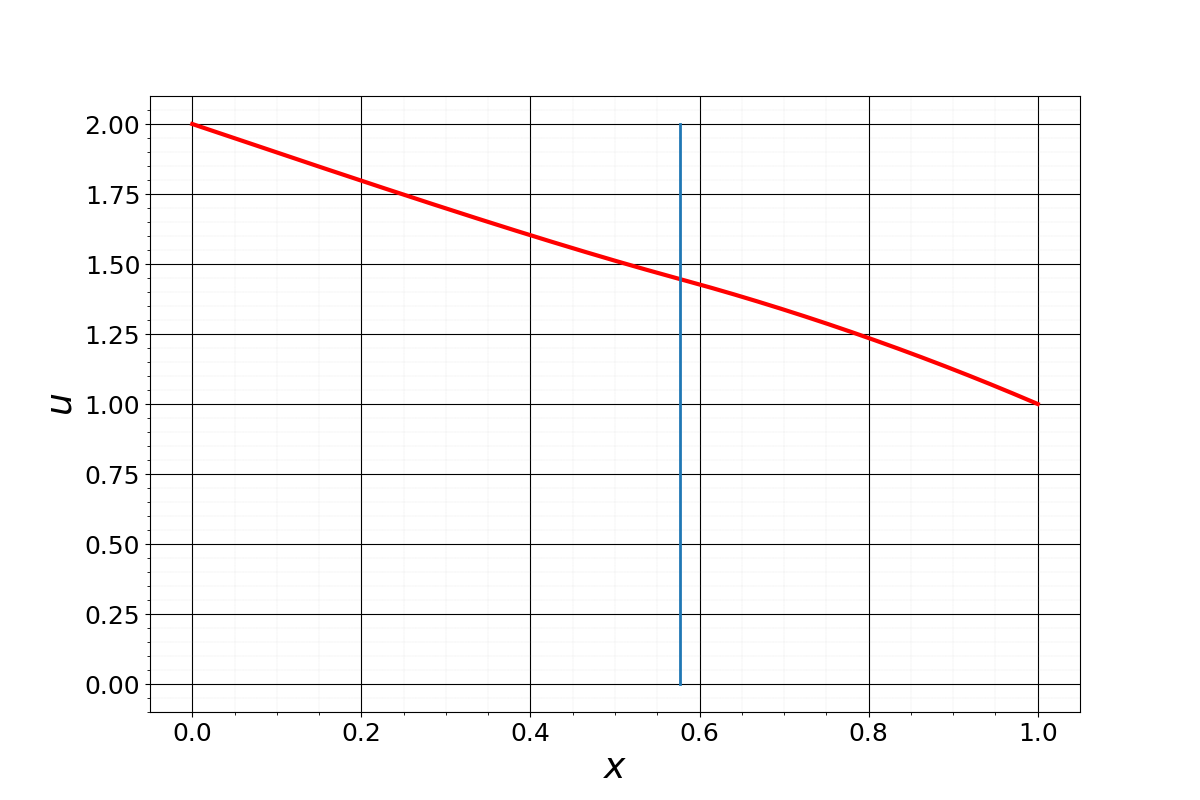
\includegraphics[width=0.85\linewidth]{Pictures/Solution.png}
			\caption{График решения. Красным -- само решение; синим -- точка разрыва}
		\end{figure}
	
		Если посмотреть ближе, то, очевидно, увидим последствия разрыва:
		\begin{figure}[h!]
			\centering
			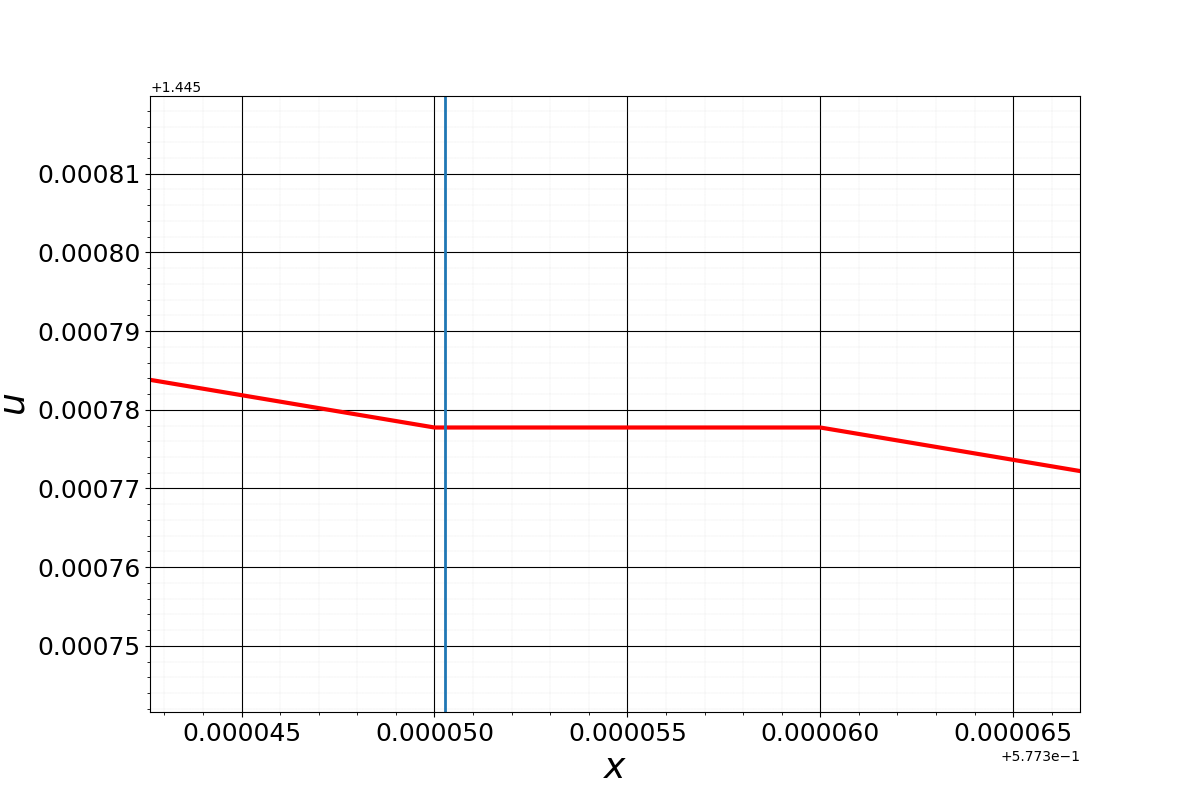
\includegraphics[width=0.85\linewidth]{Pictures/Scaled.png}
			\caption{Увеличенный график}
		\end{figure}
	
		
		
		\tocsection{Вывод}
		В работе был реализован метод встречных прогонок для решения краевой задачи для одномерного стационарного уравнения теплопроводности с кусочно-непрерывными коэффициентами.
		
		
\end{document}